\documentclass[12pt,letterpaper]{report}
\usepackage[utf8]{inputenc}
\usepackage{amsmath}
\usepackage{amsfonts}
\usepackage{amssymb}
\usepackage{graphicx}
\author{Tyler Anderson}
\title{Bipolar Coordinates}
\begin{document}
\section*{Coordinate Conversion}

First off, things are complicated because this machine doesn't truly use polar coordinates. Normal polar coordinates consist of an angle and a distance ($\theta$ and r). But in our case, the extruder arms move in an arc and not a straight line. This means that our coordinates have to be represented by two angles. $\theta_1$ is the angle of rotation of the platter. $\theta_2$ is the angle of the arm. Since this system has two poles, we'll call it bipolar coordinates. 

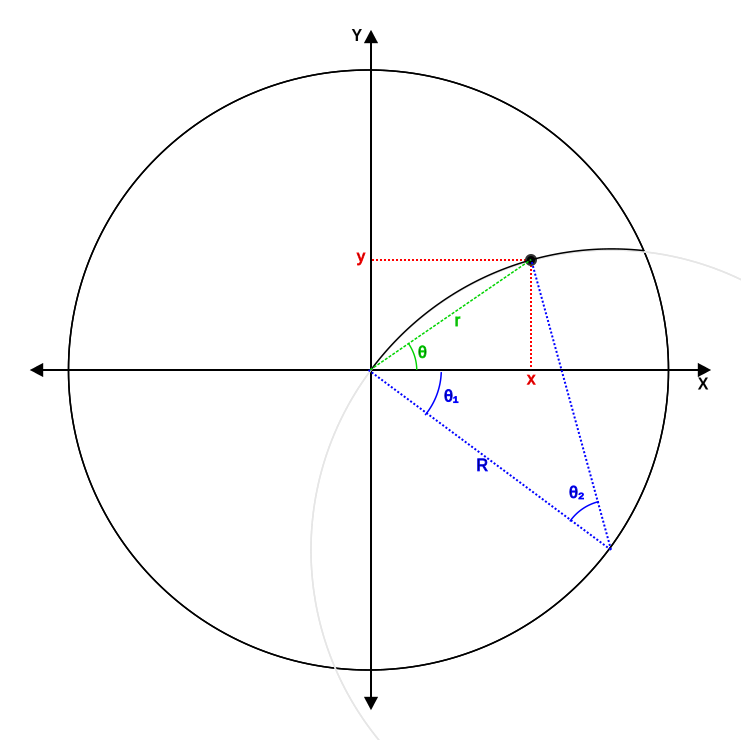
\includegraphics[width=4in]{polar.png}

In the above diagram, R is the length of the extruder arm which is 160mm on this machine. To simplify calculations all angles will be in radians.

The normal conversion from cartesian to polar is given by \ldots
\begin{equation}
	\theta = tan^{-1} \left( \dfrac{y}{x} \right)  
\end{equation}
\begin{equation}
	r = \sqrt{x^{2}+y^{2}}
\end{equation}

But for bipolar coordinates the conversion is \ldots
\begin{equation}
	\theta_2 = 2 sin^{-1} \left( \dfrac{\sqrt{x^2+y^2}}{2R} \right)
\end{equation}
\begin{equation}
	\theta_1 = \dfrac{\pi-\theta_2}{2} - tan^{-1} \left( \dfrac{y}{x} \right) 
\end{equation}

\section*{Parametric Equations}
We can now convert coordinates directly from cartesian to bipolar form, but more importantly, we need to know how to make the machine move in a straight line. Motion in 2D space is described using parametric equations. The equations for moving in a straight line in cartesian space are \ldots
\begin{equation}
	x = V_x t + x_0
\end{equation}
\begin{equation}
	y = V_y t + y_0
\end{equation}
\ldots where t is time, $V_x$ \& $V_y$ are the velocities in the $x$ and $y$ directions, and $x_0$ \& $y_0$ are the starting points.

By substituting these into the conversion for bipolar coordinates, we get the equations for linear motion in bipolar space.
\begin{equation}
	\theta_2 = 2 sin^{-1} \left(  \frac{\sqrt{(V_xt+x_0)^2 + (V_yt+y_0)^2}}{2R} \right)
\end{equation}
\begin{equation}
	\theta_1 = \frac{\pi-\theta_2}{2R} - tan^{-1} \left( \frac{V_y t + y_0}{V_x t + x_0} \right)
\end{equation}

\section*{Time}
The axes on the machine are controlled by stepper motors. Unlike most electric motors which run continuously when they are turned on, stepper motors move in small increments. In order to drive the motors, the controller needs to know exactly when to make each step. Since we know what the location of each axis will be after each step, we can solve for $t$ in the parametric equations to find out when to pulse the motors.

For $\theta_2$ the parametric equation is parabolic, so we must use the quadratic formula. The solution is broken down into components for simplicity.
\begin{equation}
	t_2 = \frac{-b\pm\sqrt{b^2-4ac}}{2a}
\end{equation}
\begin{equation}
	a = V_x^2+V_y^2
\end{equation}
\begin{equation}
	b = 2(V_x x_0 + V_y y_0)
\end{equation}
\begin{equation}
	c = x_o^2 + y_0^2 - 4R^2sin^2 \left( \frac{\theta_2}{2} \right)
\end{equation}

Remember that in the above equations, $\theta_2$ is the point after the next step will be made. It is easily determined by
\begin{equation}
	\theta_{2,n+1} = \theta_{2,n} \pm \Delta\theta_2
\end{equation}
where $\Delta\theta_2$ is the distance that axis moves with each step. $\Delta\theta_2$ is governed by the gear ratio and the number of steps per revolution of the motor.

The reason for the $\pm$ above is because we do not know in which direction the axis is moving (forward or backward) or if it will reverse direction before the step occurs. This means there are two possibilities. Combined with the two possible outcomes of the quadratic, this means that we can get up to 4 values for $t_2$. So which one do we choose? We use the lowest value that is still in the future ($> t$).

Now lets solve for $t$ in $theta_1$
\begin{equation}
	t_1 = \frac{x_0 * tan\left( \frac{\pi-\theta_2}{2} - \theta_1 \right) - y_0}{v_y - v_x * tan\left( \frac{\pi-\theta_2}{2} - \theta_1 \right)}
\end{equation}

But there is a problem. $\theta_1$ is dependent on $\theta_2$. In order to find $t$ we need to know $\theta_2$, but in order to get $\theta_2$ we need to know $t$. The solution we used is crude but effective. Instead of waiting until a certain time to make the step, the software periodically checks what the position of $\theta_1$ should be based on the current time. If the difference between the current and ideal positions is too great, it makes the step.

\section*{Derivatives}
It is also important for the software to know in which direction to move the motors, forward or reverse. When moving in a straight line in cartesian space, the direction is always the same. But in bipolar space, the direction can reverse in the middle of a move. In order to determine which way to go, we must find the signs of the derivatives of the parametric equations.

These are the derivatives. Here $x$ and $y$ are given by equations (5) and (6).
\begin{equation}
	\dfrac{d\theta_2}{dt} = \dfrac{2V_xx+2V_yy}{2R\sqrt{x^2+y^2}\sqrt{1-\dfrac{x^2+y^2}{4R^2}}}
\end{equation}
\begin{equation}
	\dfrac{d\theta_1}{dt} = -\left( \dfrac{1}{1-\dfrac{x^2+y^2}{4R^2}} \right) \left( \dfrac{(V_x^2+V_y^2)t+x_0V_x+y_0V_y}{2R\sqrt{x^2+y^2}} \right) - \left( \dfrac{1}{1+\left(\dfrac{y}{x}\right)^2} \right) \left( \dfrac{V_yx_0-V_xy_0}{x^2} \right) 
\end{equation}
\end{document}]{article}